\documentclass[a4paper,11pt,titlepage]{article}
\usepackage{graphicx}
\author{Abrie Greeff\\B.Sc Hons (Computer Science)\\Department of Computer Science\\University of Stellenbosch}
\title{Simulation Project 1}
\begin{document}
\maketitle
\section{Introduction}
The purpose of this project is to model and simulate the behaviour of an optical network consisting of optical packet switching (OPS) using a set of M/M/L/k queues. A basic network topology will be examined. The network will consist of four OPS nodes and eight access nodes (ANs). Each OPS node is connected to two other OPS nodes in a grid topology and also to two ANs. Each OPS node has 16 bi-directional ports that can be used as channel links or re-circulation ports. This project will simulate wavelength channel lengths between one and four. Tests will also be conducted on different probabilities of packets being generated at each AN.
\section{Implementation}
The application that was developed for this simulation was written in Java 1.5. Three variables needs to be determined before each simulation can be done. These are the amount of time steps the simulation should run, the probability that a packet is generated, and the length of the wavelength channel.

The network was setup to look like Fig.~\ref{fig:topo}.
\begin{figure}[htbp]
	\centering
	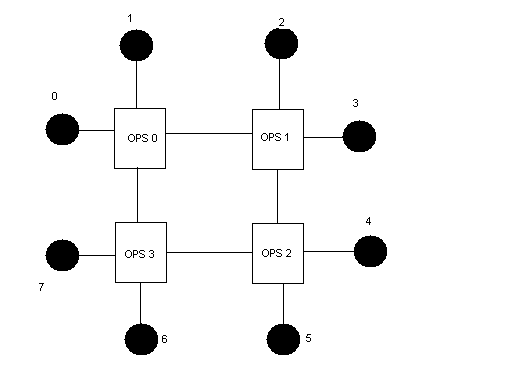
\includegraphics[width=10cm]{topo.png}
	\caption{Network Topology}
	\label{fig:topo}
\end{figure}
In every time step the following steps are followed. First all the OPS nodes are checked to see if they have any packets that must be moved to other OPS nodes. These packets are then delivered to their targets. The ANs are then checked if they generated any packets that must be sent to the OPS nodes. If a packet was created it is sent to the OPS node the AN connects to.
\section{Simulations}
The following results were obtained from different simulations of the input parameters.\\
\begin{tabular}{|c|c|c|c|c|c|c|}
\hline
	Time & Packets & Recieved & Dropped & Drop Rate & Wave & Prob\\
\hline
	500 & 	428		&		427			&	0				&	0.0\%			&	1		&		0.1\\
	500 & 	1190	&		722			&	448			&	38.29\%		&	1		&		0.3\\
	500 & 	2012	&		578			&	1397		&	70.73\%		&	1		&		0.5\\
	500 & 	2857 	&		454			&	2362		&	83.87\%		&	1		&		0.7\\
	500 & 	4008	&		431			&	3532		&	89.12\%		&	1		&		1.0\\
\hline
	500 & 	424		&		315			&	79			&	20.05\%		&	2		&		0.1\\
	500 & 	1210 	&		590			&	589			&	49.95\%		&	2		&		0.3\\
	500 & 	2044	&		745			&	1268		&	62.99\%		&	2		&		0.5\\
	500 & 	2828	&		824			&	1972		&	70.52\%		&	2		&		0.7\\
	500 & 	4008	&		829			&	3147		&	79.149\%	&	2		&		1.0\\
\hline 
	500 & 	392		&		276			&	102			&	26.98\%		&	3		&		0.1\\
	500 & 	1195	&		587			&	593			&	50.25\%		&	3		&		0.3\\
	500 & 	1981	&		738			&	1227		&	62.44\%		&	3		&		0.5\\
	500 & 	2816	&		815 		&	1985		&	70.89\%		&	3		&		0.7\\
	500 & 	4008  &		845 		&	3147		&	78.83\%		&	3		&		1.0\\
\hline 
	500 & 	437 	&		313			&	122			&	28.04\%		&	4		&		0.1\\
	500 & 	1219	&		548			&	631			&	51.93\%		&	4		&		0.3\\
	500 & 	2000  &		732 		&	1264		&	63.32\%		&	4		&		0.5\\
	500 & 	2840	&		811 		&	2025		&	71.4\%		&	4		&		0.7\\
	500 & 	4008 	&		854 		&	3150		&	78.67\%		&	4		&		1.0\\
\hline  
\end{tabular}
\section{Conclusion}
The amount of packets that are lost over time are not satisfactory. In these circumstances it will be wise to decide what the load on the network you are designing this setup for is. If the network is to expect low packet activity a OPS with a wavelength channel of one is the best choice. In circumstances where high packet activity is to be expected an OPS with wavelength channel four would be the best.
\end{document}
